\documentclass[UTF8]{ctexart}

% 导言区

% 标题、作者、日期
\title{Your Paper}
\author{You}
\date{\today}
% 加载宏包
% 插入链接
% \usepackage{hyperref}[colorlinks, linkcolor=blue]
\usepackage[colorlinks=true, allcolors=blue]{hyperref}
% 使用 AMS-LaTex 提供的数学功能
\usepackage{amsmath}
% 插入图片
\usepackage{graphicx}
\graphicspath{{Figures/}}
% 版面设置
% 页边距
\usepackage{geometry}
\geometry{papersize={20cm, 15cm}}
\geometry{left=1cm,right=2cm,top=3cm,bottom=4cm}
% 页眉页脚
\usepackage{fancyhdr}
\pagestyle{fancy}
\lhead{\author}
\chead{\date}
\rhead{xxxx}
\lfoot{}
\cfoot{\thepage}
\rfoot{}
\renewcommand{\headrulewidth}{0.4pt}
\renewcommand{\headwidth}{\textwidth}
\renewcommand{\footrulewidth}{0pt}
% BibLaTex
\usepackage[backend=biber]{biblatex}
\addbibresource{ref.bib}
% \usepackage[style=apa]{biblatex} % biber
% \usepackage{cite} 
% The cite package, which is meant to be used with BibTeX and a suitably chosen \bibliographystyle, 
% provides tools to manage the typeset format of numeric-style citation call-outs. 
% The biblatex package can generate numeric citation call-outs as well, but it uses mechanisms that are incompatible with cite. 

% 正文区
\begin{document}
    \maketitle  % 控制序列:显示导言区中定义的标题、作者、日期
    使用 titling 宏包可以修改上述默认格式,参考 \href{https://texdoc.org/serve/titling.pdf/0}{Texdoc-titling}

    % 插入目录:保存并用 XeLaTex 编译两次
    \tableofcontents

    \section{This is a section}
    section example

    \subsection{This is a sub section}
    subsection example

    \subsubsection{This is a sub sub section}
    subsubsection example

    \paragraph{This is a paragraph}
    paragraph example

    \subparagraph{This is a sub paragraph}
    subparagraph example

    \section{数学公式示例}

    这是一个行内公式:Einstein 's $E=mc^2$. 行内公式的标点应该放在数学模式的限定符之外

    \[ E=mc^2. \]

    这是一个行间公式:

    \begin{equation}
    E=mc^2.
    \end{equation}

    行间公式的标点应该放在数学模式限定符之内

    \section{插入图片与表格}

    \subsection{图片}
    显示在 Tex 源文件同目录下的 Qomolangma.jpg 图片
    
    可选控制参数,图片宽度被缩放至页面宽度的百分之八十,而高度会按比例缩放

    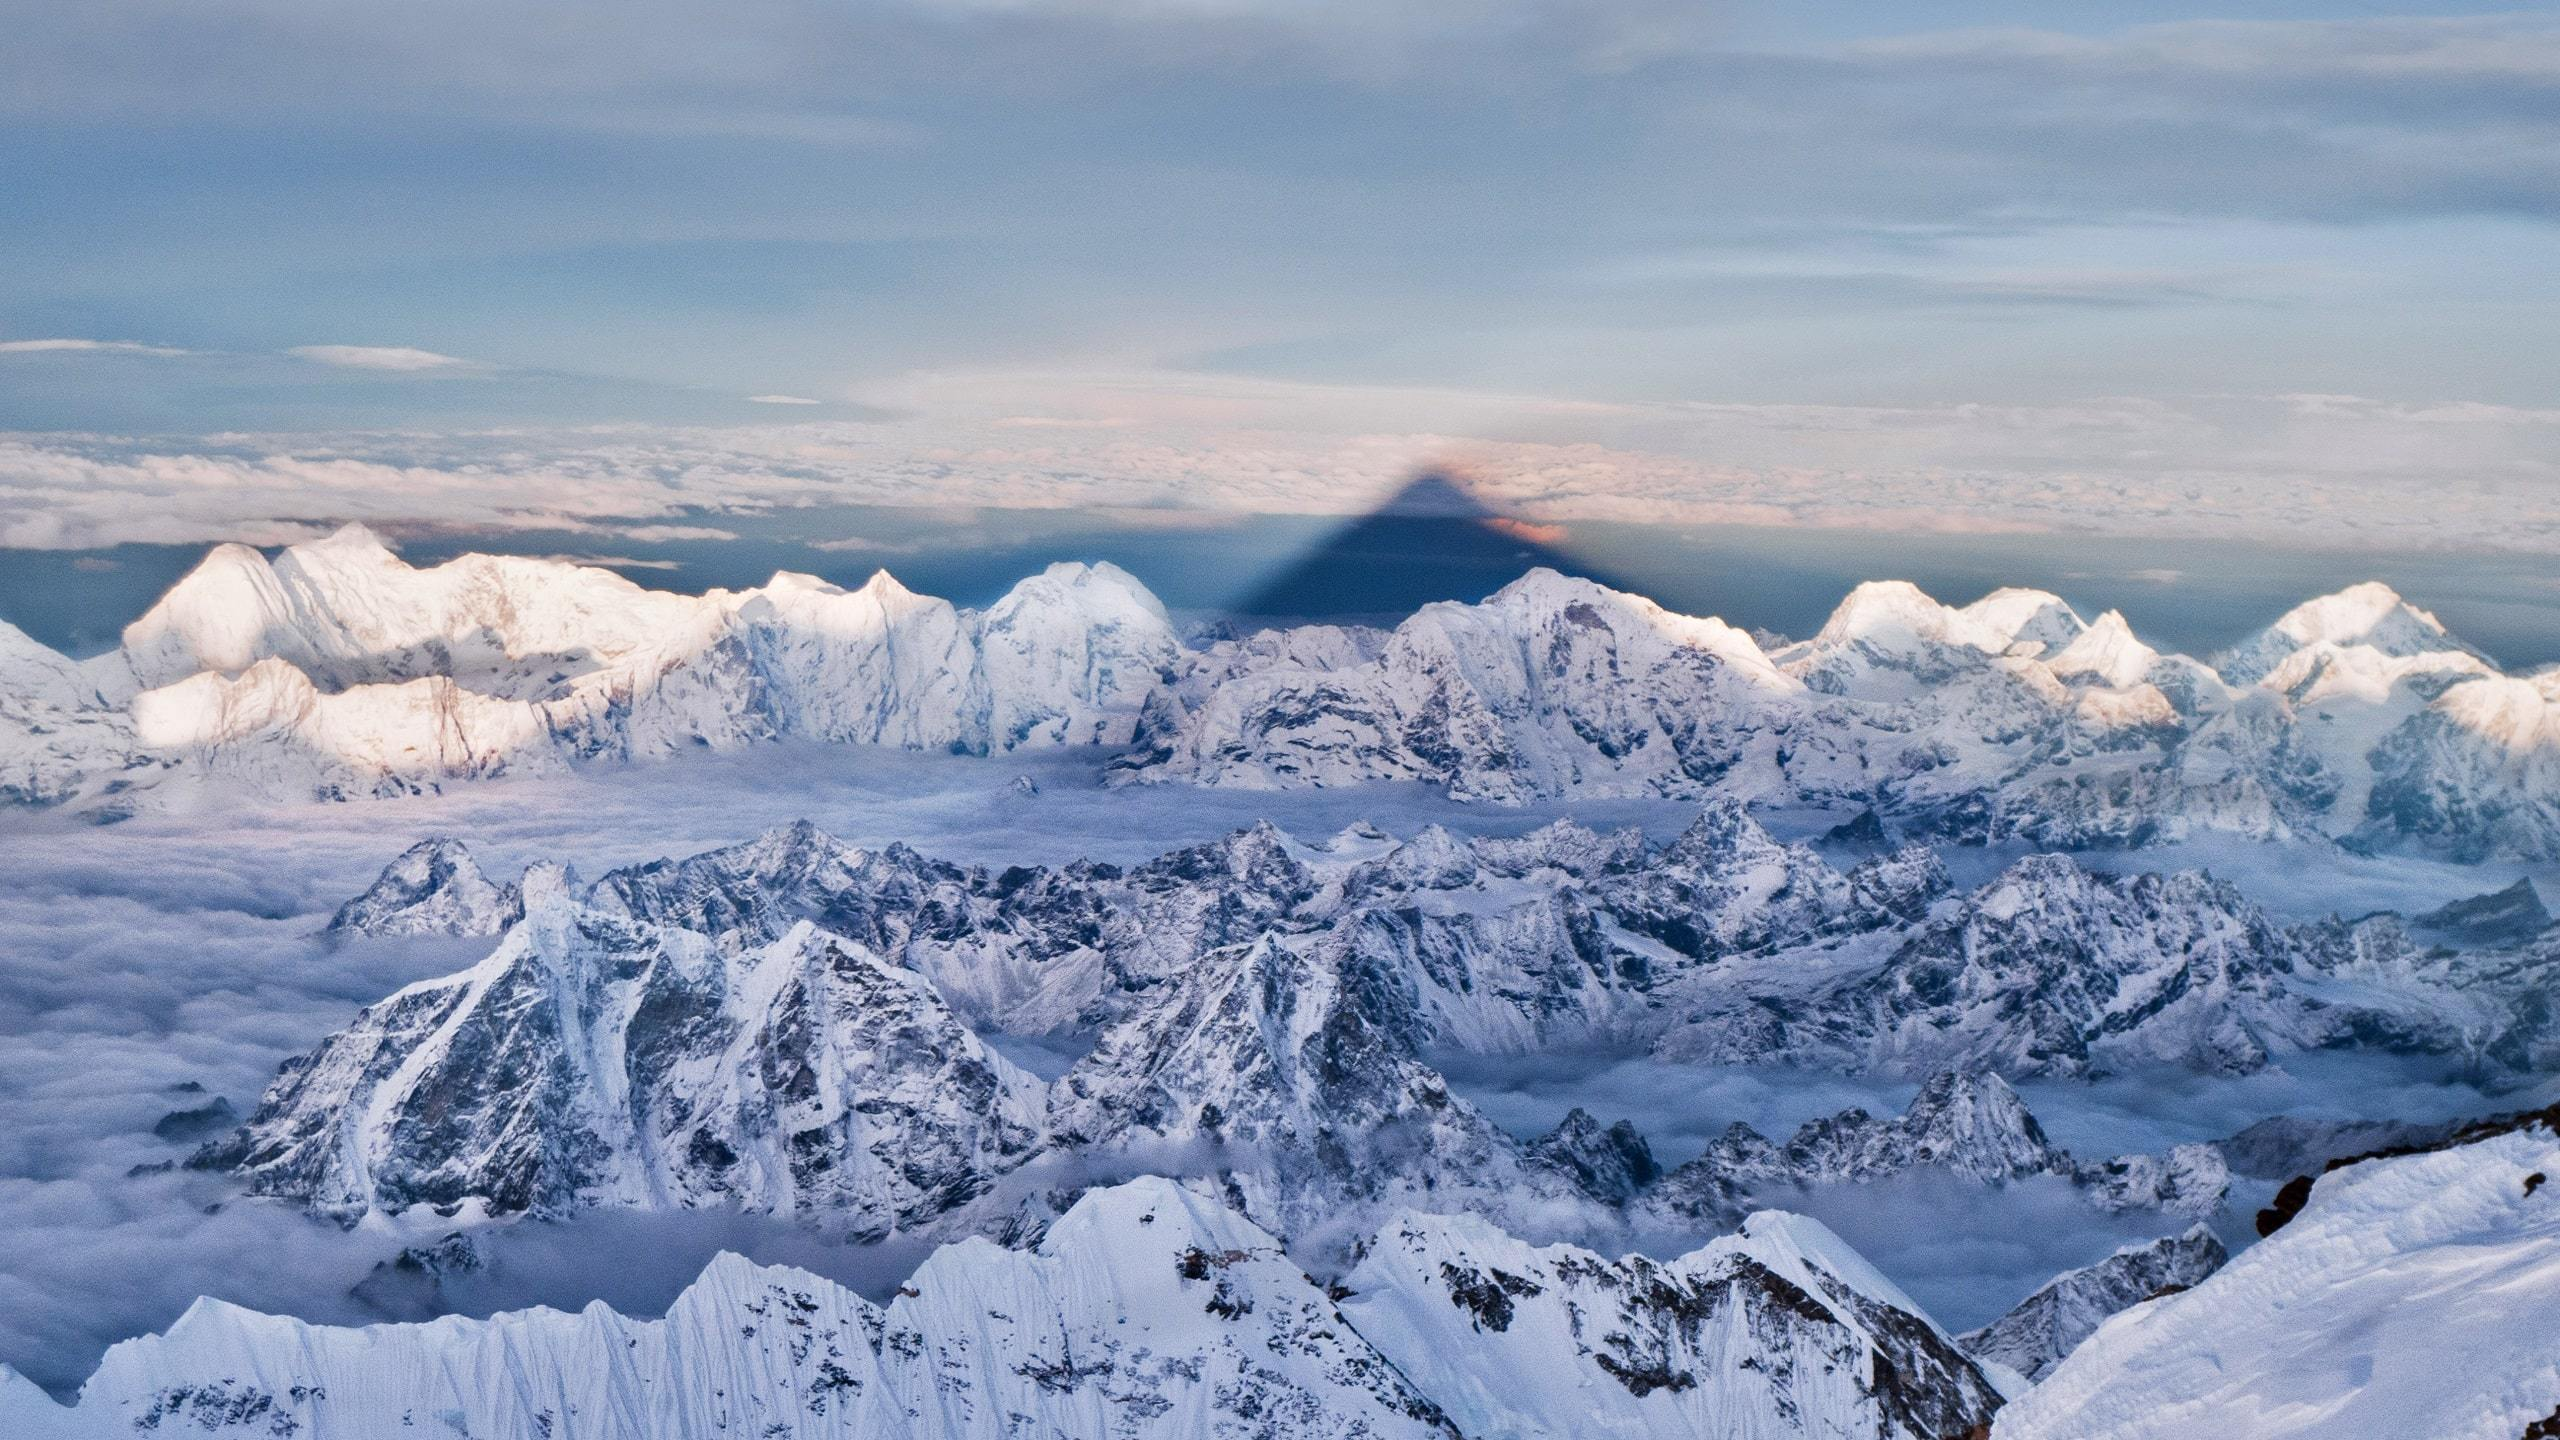
\includegraphics[width = .8\textwidth]{Qomolangma.jpg}

    可查看 graphicx 宏包的文档: \href{https://texdoc.org/serve/graphicx.pdf/0}{Texdoc-graphicx}

    \subsection{表格}
    这是一个表格

    \begin{tabular}{|l|c|r|}
         \hline
        操作系统& 发行版& 编辑器\\
        \hline
        Windows & MikTeX & TexMakerX \\
        \hline
        Unix/Linux & teTeX & Kile \\
        \hline
        Mac OS & MacTeX & TeXShop \\
        \hline
        通用& TeX Live & TeXworks \\
        \hline
    \end{tabular}

    \subsection{浮动体}
    浮动体:自动调整位置的环境

    \begin{figure}[htbp]
        \centering
        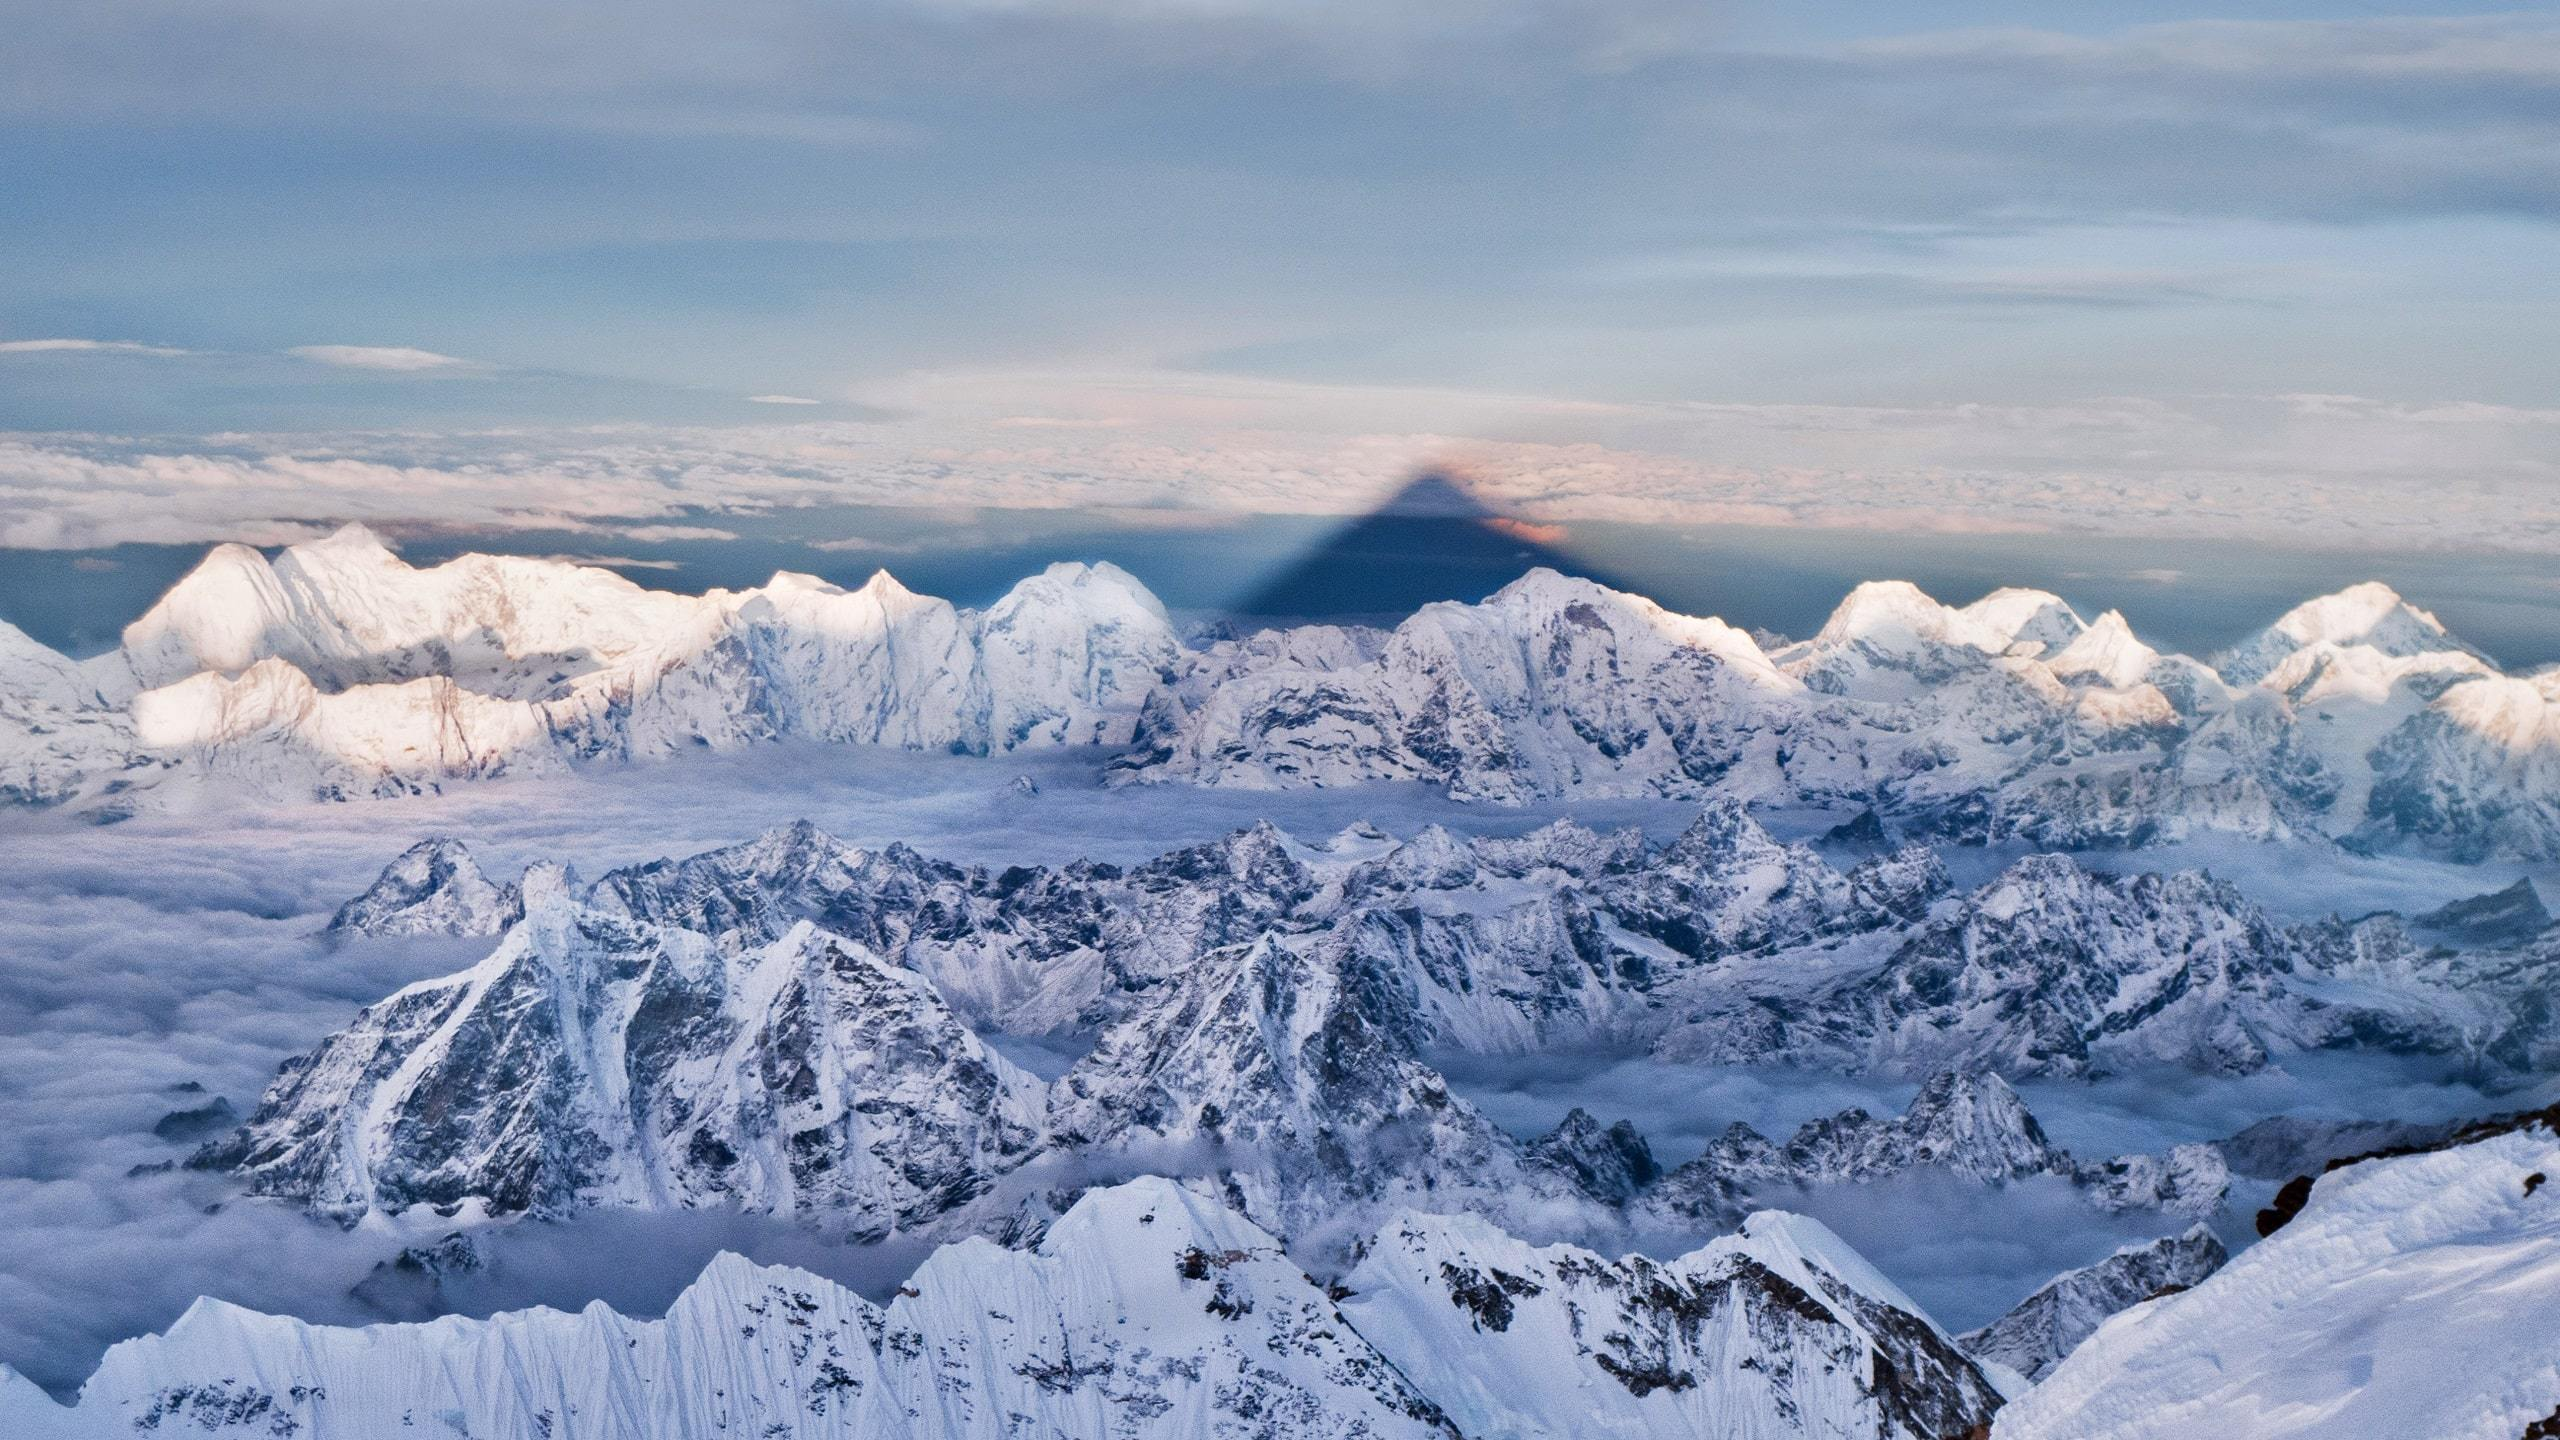
\includegraphics[width = .5\textwidth]{Qomolangma.jpg}
        \caption{珠穆朗玛峰的影子}
        \label{fig::Qomolangma}
    \end{figure}

    \section{参考文献}
    添加参考文献的方法

    \subsection{不使用 bibtex / biber }
    %\iffalse
    % 99 代表参考文献的个数最大为 99
    \begin{thebibliography}{99}  
        \bibitem{ref1}Zheng L, Wang S, Tian L, et al., Query-adaptive late fusion for image search and person re-identification, Proceedings of the IEEE Conference on Computer Vision and Pattern Recognition, 2015: 1741-1750.  
        \bibitem{ref2}Arandjelović R, Zisserman A, Three things everyone should know to improve object retrieval, Computer Vision and Pattern Recognition (CVPR), 2012 IEEE Conference on, IEEE, 2012: 2911-2918.  
        \bibitem{ref3}Lowe D G. Distinctive image features from scale-invariant keypoints, International journal of computer vision, 2004, 60(2): 91-110.  
        \bibitem{ref4}Philbin J, Chum O, Isard M, et al. Lost in quantization: Improving particular object retrieval in large scale image databases, Computer Vision and Pattern Recognition, 2008. CVPR 2008, IEEE Conference on, IEEE, 2008: 1-8.  
    \end{thebibliography}

    引用参考文献的方法:

    在正文中使用\cite{ref1},比如\cite{ref1, ref4}
    %\fi
    \subsection{使用 bibtex / biber }
    上标且带方括号的引用标记 \cite{greenwade93}

    带方括号的引用标\parencite{greenwade93}

    无格式化的引用标\supercite{yerlanova2021high}

    \printbibliography

\end{document}